\documentclass[12pt]{report}
\usepackage[hidelinks]{hyperref}
\usepackage[T1]{fontenc}
\usepackage[utf8]{inputenc}
\usepackage[turkish,english,shorthands=:!]{babel}
\usepackage{apacite}
%%% left: 40mm, top: 25mm, right: 25mm, bottom: 25mm
\usepackage[a4paper,left=40.2mm,top=24.2mm,right=25.4mm,bottom=36mm]{geometry}
\usepackage{epigraph}
\usepackage{graphicx}
\usepackage{float}
\usepackage[font={footnotesize,bf}]{caption}
\usepackage[font={footnotesize,bf}]{subcaption}
\usepackage{wrapfig}
\usepackage[usenames,dvipsnames]{color}
\usepackage[titletoc,title]{appendix}
\usepackage{afterpage}
\usepackage[doublespacing]{setspace}
\usepackage{tocloft}
\usepackage{url}
\usepackage{indentfirst}

%%% For dummy texts, you can remove it.
\usepackage{lipsum}

%%% Turning off all figures, required for turnitin upload to reduce the size of the document.
%%% Remove the next two lines if you want the figures at their place
%\usepackage[figuresonly,nolists,nomarkers]{endfloat}
%\renewcommand{\processdelayedfloats}{}

%%% Same fonts for URL
\AtBeginDocument{\urlstyle{APACsame}}

%%% Figure and Table counters
\usepackage{chngcntr}
\counterwithout{figure}{chapter}
\counterwithout{table}{chapter}


%****************************************
% SPACING

%%% Footnote line spacing
\setlength{\footnotesep}{\baselineskip}

%%% Adding extra space between paragraphs
\setlength{\parskip}{0.5\baselineskip}
%........................................


%****************************************
% BIBLIOGRAPHY

%%% Bibliography line spacing
\usepackage{natbib}
\setlength{\bibsep}{0.0pt}

%%% Removing parentheses around year in bibliography
\AtBeginDocument{
\renewcommand{\BBOP}{}
\renewcommand{\BBCP}{}
}

%%% Adding ":" character before page number in citations
\bibpunct[: ]{(}{)}{:}{a}{,}{~}
%........................................


%****************************************
% BLOCK QUOTES

%%% Spaces before and after block quotes
\usepackage{etoolbox}
\AtBeginEnvironment{quote}{\vspace{-\baselineskip}}
\AtEndEnvironment{quote}{\vspace{-\baselineskip}}

%%% Spaces before and after block quotes, indentation
\renewcommand{\quote}{\list{}{\rightmargin=4em\leftmargin=4em}\item\relax}

%%% Spacing
\expandafter\def\expandafter\quote\expandafter{\quote\singlespacing}
%........................................


%****************************************
% CHAPTERS

%%% Chapter titles
\usepackage{titlesec}
\titleformat{\chapter}[display]
        {\normalfont\fontsize{14pt}{14pt}\centering\bfseries}{\MakeUppercase{\chaptertitlename}\  \thechapter}{2\baselineskip}{\uppercase}
\titleformat*{\section}{\bfseries\fontsize{12pt}{12pt}}
\titleformat*{\subsection}{\bfseries\fontsize{12pt}{12pt}}

%%% Chapter title spacing
%%% Centered, Top: 50mm, Next: 3 line after
\titlespacing{\chapter}{0pt}{13mm}{3\baselineskip} 

%%% Bibliography title spacing
%%% Centered, Top: 50mm, Next: 4 line after
\titlespacing*{name=\chapter,numberless}{0pt}{16mm}{4\baselineskip} 

%%% RENAMING CHAPTER TITLES
\addto\captionsenglish{%
  \renewcommand{\contentsname}{\MakeUppercase{Table of Contents}}%
  \renewcommand{\listtablename}{\MakeUppercase{List of Tables}}%
  \renewcommand{\listfigurename}{\MakeUppercase{List of Figures}}%
  \renewcommand{\bibname}{\MakeUppercase{Bibliography}}%
}
%........................................


%****************************************
% EPIGRAPH

%%% Epigraph setup
\setlength{\epigraphwidth}{.65\textwidth}
\setlength{\epigraphrule}{0pt}
%........................................


%%% PDF setup
\hypersetup{
    pdftitle	= {MFA Thesis},
    pdfauthor	= {Mustafa ilhan},
    pdfsubject	= {Trash, Art, Transformation},
    pdfkeywords	= {mfa thesis, trash, art, transformation},
    colorlinks	= false,
    pdfborder	= {0 0 0},
    pdfpagemode	= UseOutlines
}


%%% Utilities
\providecommand{\quotes}[1]{``#1''}
\providecommand{\singlequotes}[1]{`#1'}


%****************************************
% BEGIN
\begin{document}
\pagenumbering{gobble}
\selectlanguage{english}


%****************************************
% COVER
\begin{titlepage}
\singlespacing
    \begin{center}
        
        \vspace*{20mm}
        \uppercase{Transforming Trash as an Artistic Act}\\
        \vspace*{3\baselineskip}
        A Master’s Thesis\\
        \vspace*{3\baselineskip}
        by\\
        MUSTAFA İLHAN
        
        \vfill
        Department of\\
        Communication and Design\\
        İhsan Doğramacı Bilkent University\\
        Ankara\\
        January 2016
        \vspace*{28mm}
        
    \end{center}
\end{titlepage}
%........................................


%****************************************
% BLANK PAGE
\clearpage
\afterpage{\null\newpage}
\clearpage
%........................................


%****************************************
% DEDICATION
\newenvironment{dedication}
  {\clearpage           % we want a new page
   \thispagestyle{empty}% no header and footer
   \vspace*{2in}		% some space at the top 
   \centering
  }
  {\par					% end the paragraph
   \vfill
   \clearpage           % finish off the page
  }

\begin{dedication}
To my family and for those who embrace trash
\end{dedication}
%........................................


\pagenumbering{roman}


%****************************************
% TITLE PAGE
\clearpage
\thispagestyle{empty}
\singlespacing
	\begin{center}
        
        \vspace*{25mm}
        TRANSFORMING TRASH AS AN ARTISTIC ACT\\
        \vspace*{4\baselineskip}
        Graduate School of Economics and Social Sciences\\
        of\\
		İhsan Doğramacı Bilkent University\\
		\vspace*{2\baselineskip}
        by\\
       	\vspace*{2\baselineskip}
        MUSTAFA İLHAN\\
        \vspace*{3\baselineskip}
        In Partial Fulfilment of the Requirements for the Degree of\\
		MASTER OF FINE ARTS\\
        \vspace{\baselineskip}
        in\\
        \vspace{\baselineskip}
        THE DEPARTMENT OF\\
        COMMUNICATION AND DESIGN\\
       	İHSAN DOĞRAMACI BİLKENT UNIVERSITY\\
        ANKARA\\
        \vspace{\baselineskip}
        January 2016
        
	\end{center}
\clearpage
%........................................


%****************************************
% APPROVAL PAGE
\clearpage
\thispagestyle{empty}

\noindent I certify that I have read this thesis and have found that it is fully adequate, in scope and in quality, as a thesis for the degree of Master of Fine Arts in Media and Design.\\

\noindent---------------------------------\\
Assist. Prof. Dr. Ersan Ocak\\
Supervisor\\

\noindent I certify that I have read this thesis and have found that it is fully adequate, in scope and in quality, as a thesis for the degree of Master of Fine Arts in Media and Design.\\

\noindent---------------------------------\\
Prof. Dr. Mehmet Yılmaz\\
Examining Committee Member\\

\noindent I certify that I have read this thesis and have found that it is fully adequate, in scope and in quality, as a thesis for the degree of Master of Fine Arts in Media and Design.\\

\noindent---------------------------------\\
Instructor Ekin Kılıç\\
Examining Committee Member\\

\noindent Approval of the Graduate School of Economics and Social Sciences\\

\noindent---------------------------------\\
Prof. Dr. Halime Demirkan\\
Director\\

\clearpage
%........................................


%****************************************
% ENGLISH ABSTRACT
\thispagestyle{plain}
\phantomsection
\addcontentsline{toc}{chapter}{ABSTRACT}
\doublespacing
\begin{center}
	\vspace*{13mm} % Top: 50mm
	{\fontsize{14pt}{14pt}\selectfont \textbf{\MakeUppercase{Abstract}}}\\
    \vspace{\baselineskip}
    TRANSFORMING TRASH AS AN ARTISTIC ACT\\
    İlhan, Mustafa\\
    M.F.A., Department of Communication and Design\\
    Supervisor: Assist. Prof. Dr. Ersan Ocak\\
    \vspace{\baselineskip}
    January 2016
\end{center}

%%% Your Abstract
\par \lipsum[3-3]

\noindent Keywords: Transformation of Trash, Trash in Art, Trash as an Art Material.
\clearpage
%........................................


%****************************************
% TURKISH ABSTRACT
\thispagestyle{plain}
\selectlanguage{turkish}
\phantomsection
\addcontentsline{toc}{chapter}{ÖZET}
\doublespacing
\begin{center}
	\vspace*{13.5mm} % Top: 50mm
	{\fontsize{14pt}{14pt}\selectfont \textbf{\MakeUppercase{Özet}}}\\
    \vspace{\baselineskip}
    \MakeUppercase{Sanatsal Bir Eylem Olarak Atığı Dönüştürme}\\
    İlhan, Mustafa\\
    Yüksek Lisans, İletişim ve Tasarım Bölümü\\
    Tez Yöneticisi: Yrd. Doç. Dr. Ersan Ocak\\
    \vspace{\baselineskip}
    Ocak 2016
\end{center}

%%% Your Özet
\par \lipsum[2-2]

\noindent Anahtar Kelimeler: Atığın Dönüştürülmesi, Sanatta Atık, Sanatsal Malzeme olarak Atık.
\clearpage
%........................................

\selectlanguage{english}

%****************************************
% ACKNOWLEDGMENTS
\thispagestyle{plain}
\phantomsection
\addcontentsline{toc}{chapter}{ACKNOWLEDGMENTS}
\doublespacing
\begin{center}
	\vspace*{13mm} % Top: 50mm
	{\fontsize{14pt}{14pt}\selectfont \textbf{\MakeUppercase{ACKNOWLEDGMENTS}}}\\
    \vspace{3\baselineskip}
\end{center}

%%% Your Ack.
\par \lipsum[1-5]

\clearpage
%........................................


%%% Automatically generated.
%****************************************
% TABLE OF CONTENTS
\phantomsection
\addcontentsline{toc}{chapter}{TABLE OF CONTENTS}

\setcounter{secnumdepth}{3}
\setcounter{tocdepth}{3}

\renewcommand{\cftchapleader}{\cftdotfill{\cftdotsep}} % dots for chapters
\renewcommand{\cfttoctitlefont}{\MakeUppercase\hfil\bfseries\fontsize{14pt}{14pt}\selectfont}
\renewcommand\cftchapfont{\mdseries}
\renewcommand\cftchappagefont{\mdseries}
\renewcommand{\cftchappresnum}{CHAPTER\space}
\renewcommand{\cftchapaftersnum}{:}

\setlength{\cftbeforetoctitleskip}{20mm}
\setlength{\cftaftertoctitleskip}{3\baselineskip}
\setlength{\cftchapnumwidth}{7em}
%\addtolength{\cftchapnumwidth}{\cftchappresnum\cftchapaftersnum}

%%% Spacing between items
\setlength{\cftbeforesecskip}{\cftbeforechapskip}
\setlength{\cftbeforesubsecskip}{\cftbeforechapskip}

\begin{singlespace}
\tableofcontents
\end{singlespace}
\clearpage
%........................................


%%% Automatically generated.
%****************************************
% LIST OF FIGURES
\phantomsection
\addcontentsline{toc}{chapter}{LIST OF FIGURES}

%%% Spacing between items
\makeatletter
\def\@chapter[#1]#2{\ifnum \c@secnumdepth >\m@ne
	\refstepcounter{chapter}%
	\typeout{\@chapapp\space\thechapter.}%
	\addcontentsline{toc}{chapter}%
	{\protect\numberline{\thechapter}#1}%
	\else
	\addcontentsline{toc}{chapter}{#1}%
	\fi
	\chaptermark{#1}%
	\if@twocolumn
	\@topnewpage[\@makechapterhead{#2}]%
	\else
	\@makechapterhead{#2}%
	\@afterheading
	\fi}
\makeatother

\renewcommand{\cftloftitlefont}{\MakeUppercase\hfil\bfseries\fontsize{14pt}{14pt}\selectfont}
\renewcommand{\cftfigaftersnum}{.}

\setlength{\cftbeforeloftitleskip}{20mm}
\setlength{\cftafterloftitleskip}{3\baselineskip}
\setlength{\cftbeforefigskip}{\cftbeforechapskip}

\begin{singlespace}
\listoffigures
\end{singlespace}
\clearpage
%........................................


%%% If you need list of tables comment off below section.
%****************************************
% LIST OF TABLES
%\phantomsection
%\addcontentsline{toc}{chapter}{LIST OF TABLES}
%\listoftables
%........................................


\pagenumbering{arabic}


%****************************************
% CHAPTERS
\chapter{INTRODUCTION}



\begin{singlespace}
\epigraph{One can even shout out through refuse\ldots}{\hfill---Kurt Schwitters, \textit{Kurt Schwitters}, 1985}
\end{singlespace}



%%% Quotation examples:
Stav says that \quotes{[t]hey forget about it and don’t think about all the time and energy and money put into disposing of it} \citep[as cited in][]{navarro2015followingtrash}. 

\citet[11]{banash2013collage} draws attentions to the advancements in the recent history of humankind by stating that \quotes{over the course of the twentieth century, the twin developments of mass production and mass media in the capitalist economies of the [western countries] completed a total transformation of everyday life, reorienting almost every activity toward consumption.} 

\quotes{The phenomenon of waste comes clearly into focus not merely as a by-product of manufacturing processes, but rather as an integral element in cycles of production and consumption} \citep[ix]{pye2010trashculture}.

Anyone can encounter with trash in the crowded urban areas \quotes{as well as the remotest corners of the world} \citep[16]{cerny1996recycled}.

%%% Footnote example:
Trash is in the streets, in people’s home, in the sea that people swim, rotating around the globe\footnote{Satellite discards are disposed to the atmosphere and they rotate around the globe like satellites.}. Even if trash is tried to move away from people’s habitat, it is as close as the nearest waste bin.

%%% Block quotation example:
The authors of the book \textit{Rubbish: the Archeology of Garbage} give clearer definition of some these words:

\begin{quote}
\textit{Trash} refers specifically to discards that are at least theoretically dry ---newspapers, boxes, cans, and so on. \textit{Garbage} refers technically to wet discards ---food remains, yard waste, and offal. \textit{Refuse} is an inclusive term for both the wet discards and the dry. \textit{Rubbish} is even more inclusive: It refers to all refuse plus construction and demolition debris. The distinction between wet and dry garbage was important in the days when cities slopped garbage to pigs, and needed to have the wet material separated from the dry; it eventually became irrelevant, but may see a revival if the idea of composting food and yard waste catches on. \citep[9]{rathje1992rubbish}
\end{quote}

\chapter{TRASH IN CULTURE AND THEORY}



\begin{singlespace}
\epigraph{Anger is nothing compared to garbage:\\Garbage eats anger for breakfast.\\It eats all of us in the end.}{\hfill---Priscilla Uppal, \quotes{Uncle Fernando’s Garbage Triptych}}
\end{singlespace}



\lipsum[1-1]



%****************************************
\section{Throwaway Culture}

\lipsum[1-1]

%%% Figure reference example:
\textit{Fountain} (Figure \ref{fig:Duchamp_Fountaine}) is an artwork produced by Marcel Duchamp, who is notable member of provocative Dada movement. 

\begin{figure}[h!]
  \centering
  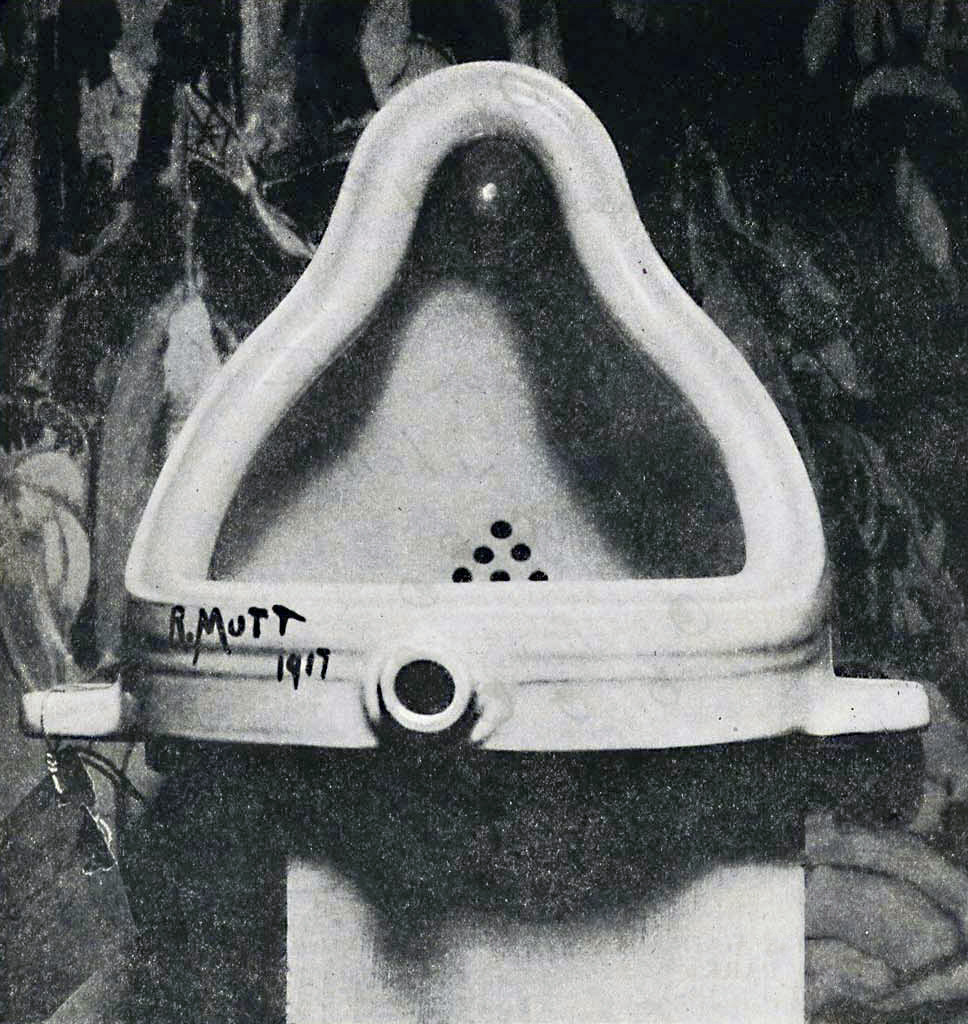
\includegraphics[height=6cm]{graphics/Duchamp_Fountaine.jpg}
  \caption{Marcel Duchamp, \textit{Fountain}, 1917, Porcelain urinal}
  \label{fig:Duchamp_Fountaine}
\end{figure}

\chapter{TRASH (IN) ART}



\begin{singlespace}
\epigraph{One day, in a rubbish heap, I found an old bicycle seat lying beside a rusted handlebar, and my mind instantly linked them together. I assembled these two objects, which everyone then recognized as a bull’s head. The metamorphosis was accomplished, and I wish another metamorphosis would occur in the reverse sense. If my bull’s head were thrown in a junk heap, perhaps one day some boy would say, \quotes{Here’s something that would make a good handlebar for my bicycle!}}{\hfill ---Pablo Picasso, \textit{Trashformations}, 1998}
\end{singlespace}



\lipsum[1-1]



%****************************************
\section{Root in the Art History}

\lipsum[1-1]


%****************************************
\section{Examples from Contemporary Artists}

\lipsum[2-2]


%****************************************
\section{The Documentary \quotes{The Gleaners and I} by Agnès Varda}

\lipsum[3-3]
\chapter{NOTEBOOKS FROM TRASHED PAPERS}



\begin{singlespace}
\epigraph{The first question I ask myself when something doesn’t seem to be beautiful is why do I think it’s not beautiful? And very shortly you discover that there is no reason. If we can conquer that dislike, or begin to like what we did dislike, then the world is more open. That path ---of increasing one’s enjoyment of life--- is the path, I think, we all best take: to use art not as self-expression, but as self-alteration; to become more open.}{\hfill---John Cage, \textit{Wild Art}, 2013}
\end{singlespace}



\lipsum[1-1]



%****************************************
\section{The Statement}

\lipsum[2-2]


%****************************************
\section{Development Progress of the Project}

\lipsum[3-3]


%****************************************
\subsection{Collecting}

\lipsum[4-4]



%****************************************
\subsection{Transformation}

\lipsum[5-5]


%****************************************
\subsection{Demonstration}

\lipsum[6-6]


%****************************************
\section{Parts of the Final Work}

\lipsum[2-2]


%****************************************
\subsection{Notebooks}

\lipsum[3-3]


%****************************************
\subsection{Exhibition}

\lipsum[4-4]



%****************************************
\subsection{Website}

\lipsum[5-5]
\chapter{CONCLUSION}



\begin{singlespace}
\epigraph{If I seem to be over-interested in junk, it is because I am, and I have a lot of it, too --- half a garage full of bits and broken pieces. I use these things for repairing other things\ldots But it can be seen that I do have a genuine and almost miserly interest in worthless objects. My excuse is that in this era of planned obsolescence, when a thing breaks I can usually find something in my collection to repair it --- a toilet, or a motor, or a lawn mower. But I guess the truth is that I simply like junk.}{\hfill---John Steinbeck, \textit{Travels with Charley, 1962}}
\end{singlespace}



\lipsum[1-2]
%........................................


%%% Automatically generated.
%****************************************
% BIBLIOGRAPHY
\nocite{*} % Add all references
\phantomsection
\addcontentsline{toc}{chapter}{BIBLIOGRAPHY}
\bibliographystyle{apacite}
\begin{singlespace}
\setlength{\bibsep}{2\itemsep}
\bibliography{literature}
\end{singlespace}
\clearpage
%........................................


%****************************************
% APPENDICES
\appendix
\phantomsection

%%% Below code is used for multiple appendices, for single appendix you need to remove code between appendices comment.
%%% remove start. [appendices]
\addtocontents{toc}{\cftpagenumbersoff{chapter}} 
\chapter*{APPENDICES}
\addtocontents{toc}{\protect\contentsline {chapter}{APPENDICES}{}{}}
\addtocontents{toc}{\cftpagenumberson{chapter}} 
%%% remove end. [appendices]

\makeatletter
\addtocontents{toc}{\let\protect\l@chapter\protect\l@section}
\makeatother

\chapter{COLLECTED MATERIALS AND MAKING OF}

\begin{figure}[h!]
  \centering
  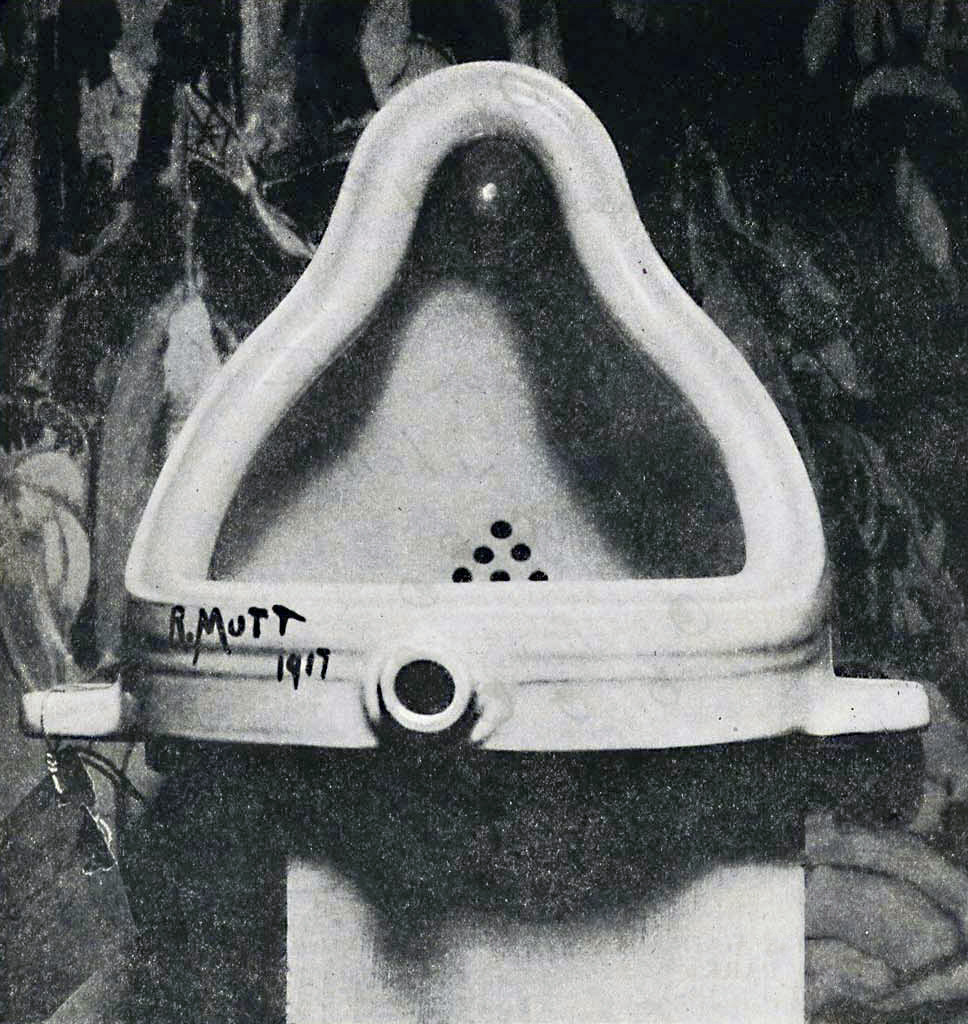
\includegraphics[height=12cm]{graphics/Duchamp_Fountaine.jpg}
  \caption{Marcel Duchamp, \textit{Fountain}, 1917, Porcelain urinal}
  \label{fig:Duchamp_Fountaine1}
\end{figure}


\begin{figure}[!tbp]
  \centering
  \begin{minipage}[b]{0.48\textwidth}
    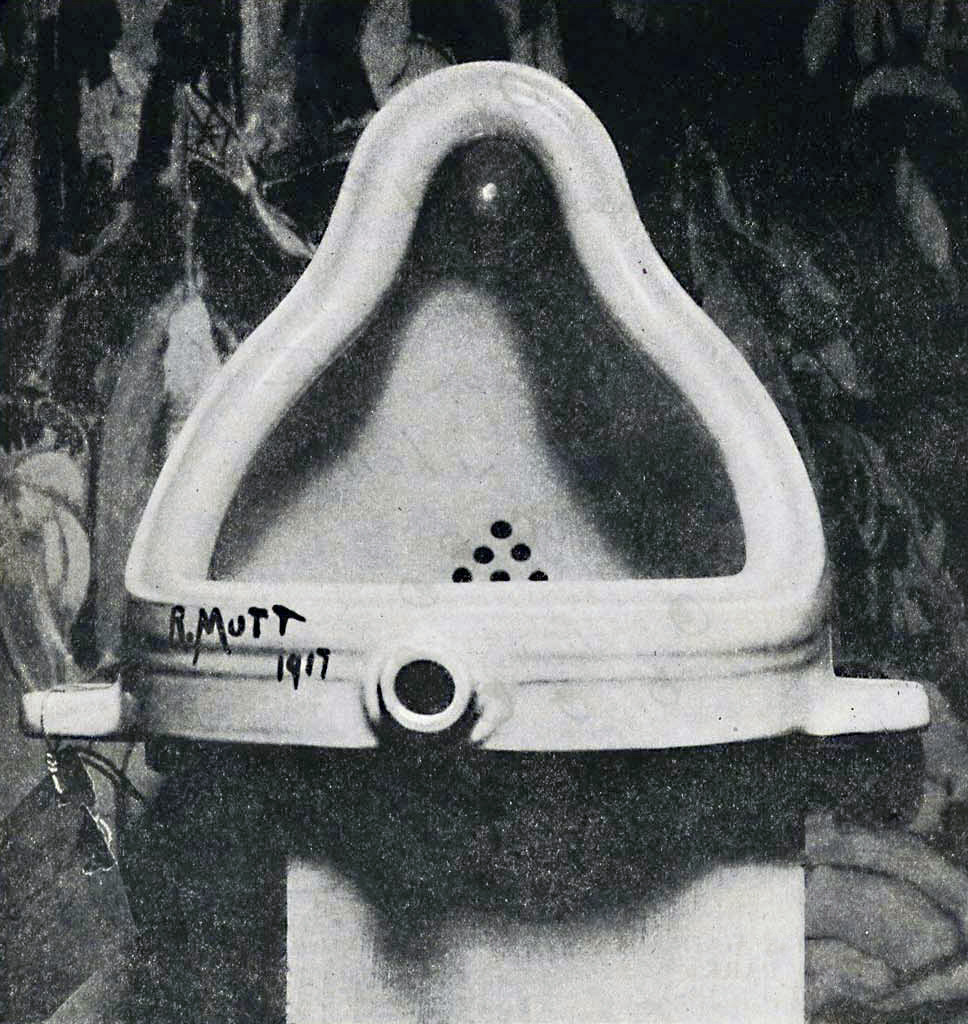
\includegraphics[width=\textwidth]{graphics/Duchamp_Fountaine.jpg}
    \caption{Marcel Duchamp, \textit{Fountain}, 1917, Porcelain urinal}
    \label{fig:Duchamp_Fountaine2}
  \end{minipage}
  \hfill
  \begin{minipage}[b]{0.48\textwidth}
    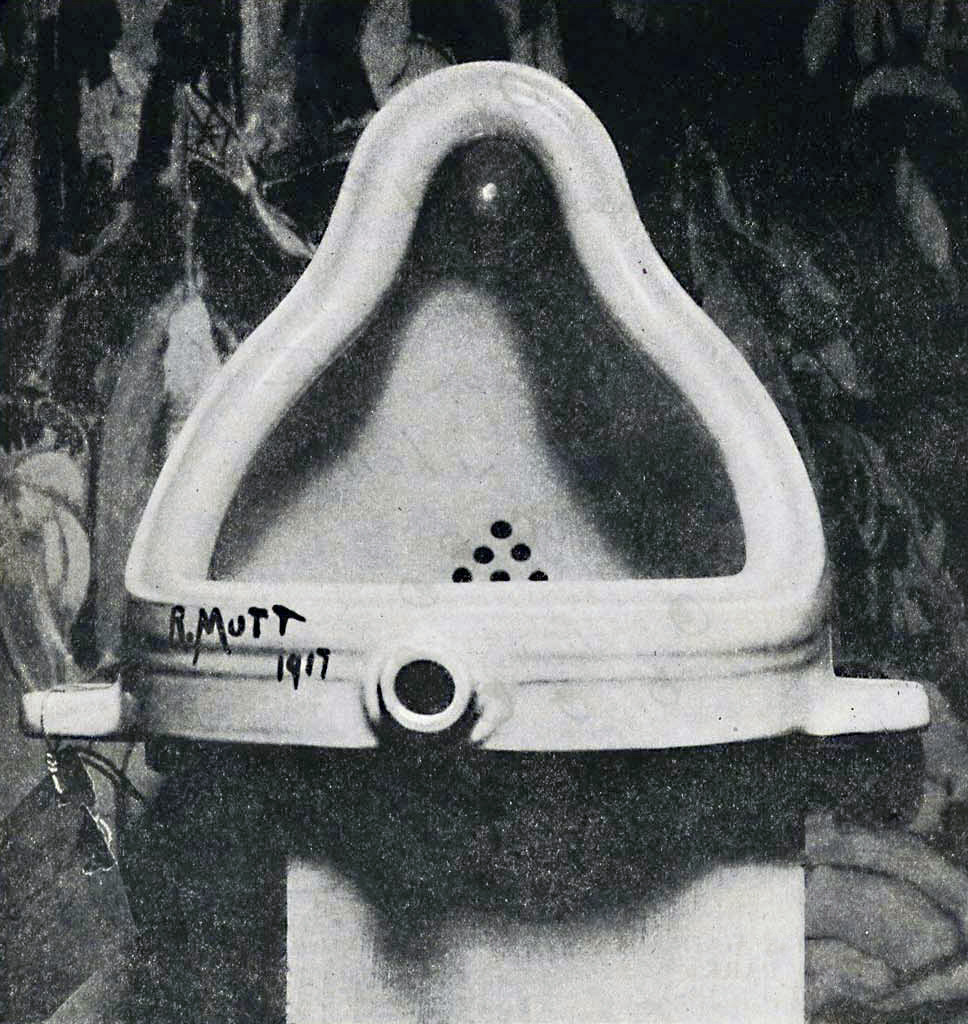
\includegraphics[width=\textwidth]{graphics/Duchamp_Fountaine.jpg}
    \caption{Marcel Duchamp, \textit{Fountain}, 1917, Porcelain urinal}
    \label{fig:Duchamp_Fountaine3}
  \end{minipage}
\end{figure}

\chapter{PHOTOGRAPHS OF FINAL WORK}

\begin{figure}[h!]
  \centering
  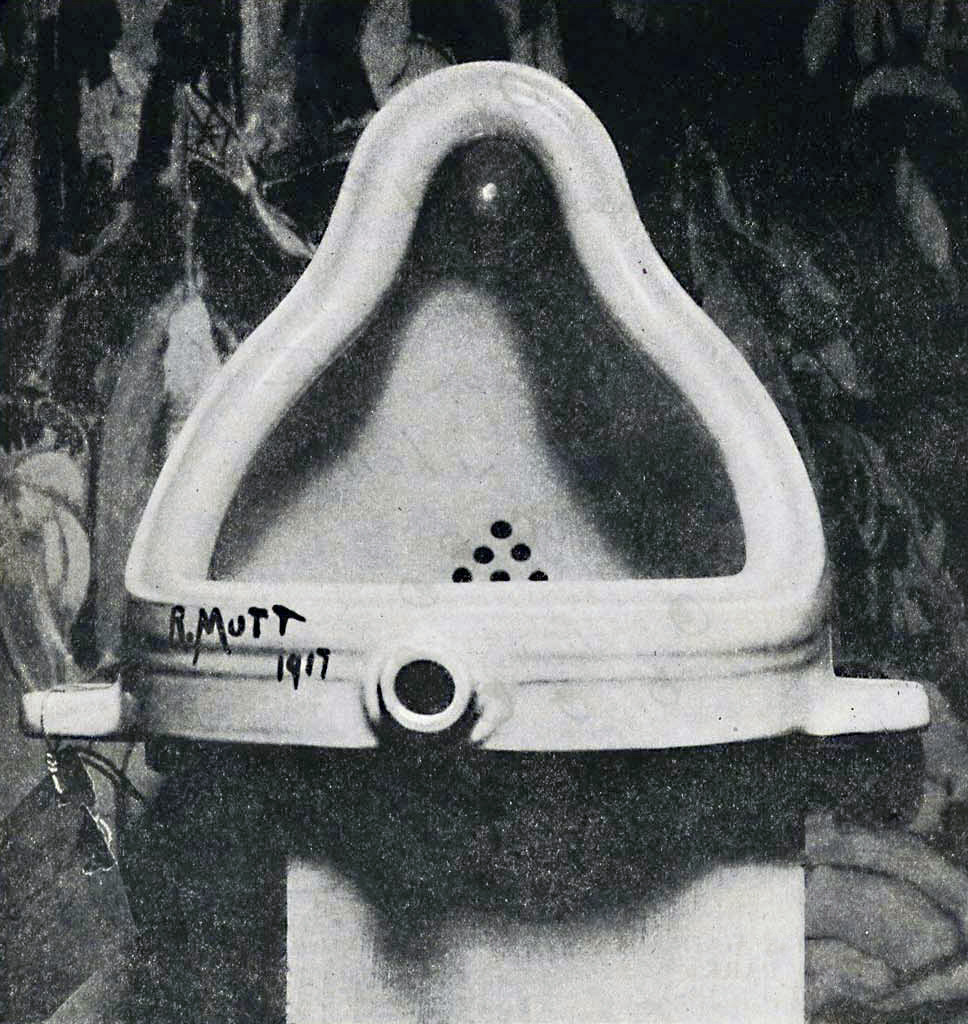
\includegraphics[height=12cm]{graphics/Duchamp_Fountaine.jpg}
  \caption{Marcel Duchamp, \textit{Fountain}, 1917, Porcelain urinal}
  \label{fig:Duchamp_Fountaine01}
\end{figure}


\begin{figure}[!tbp]
  \centering
  \begin{minipage}[b]{0.48\textwidth}
    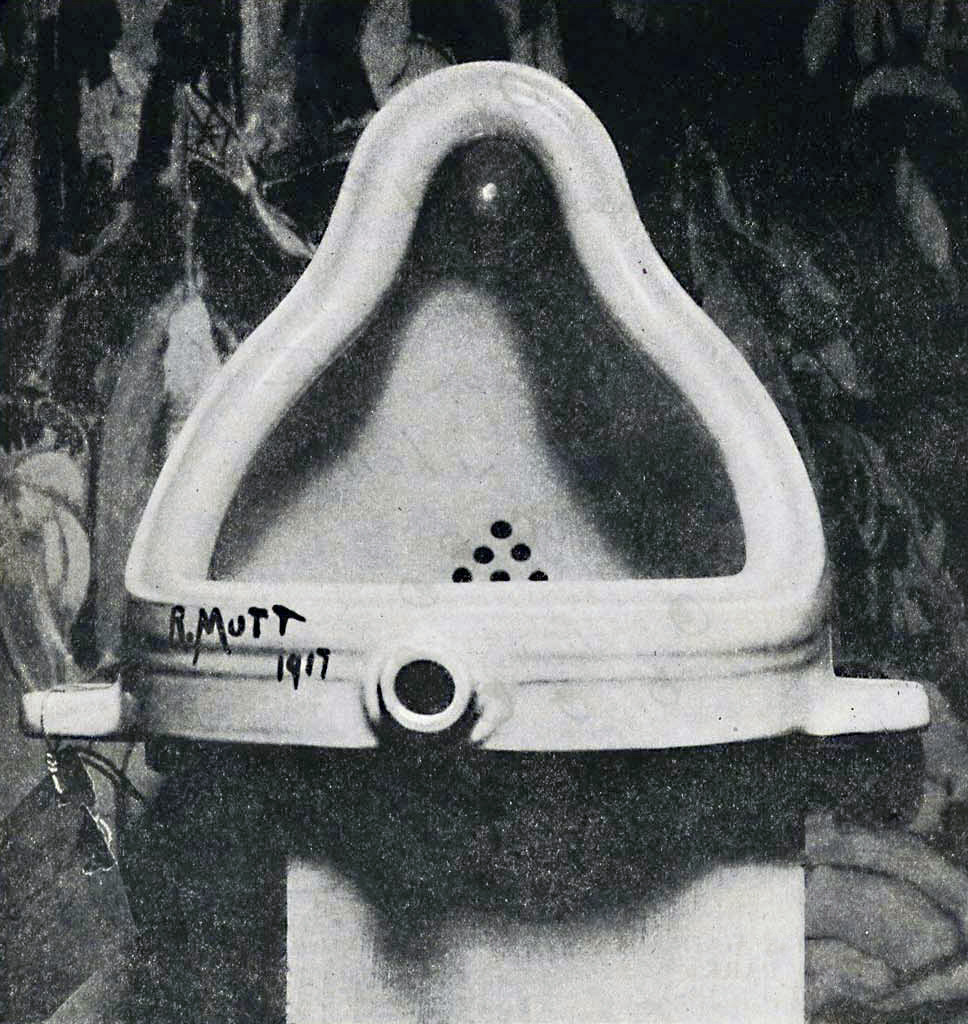
\includegraphics[width=\textwidth]{graphics/Duchamp_Fountaine.jpg}
    \caption{Marcel Duchamp, \textit{Fountain}, 1917, Porcelain urinal}
    \label{fig:Duchamp_Fountaine02}
  \end{minipage}
  \hfill
  \begin{minipage}[b]{0.48\textwidth}
    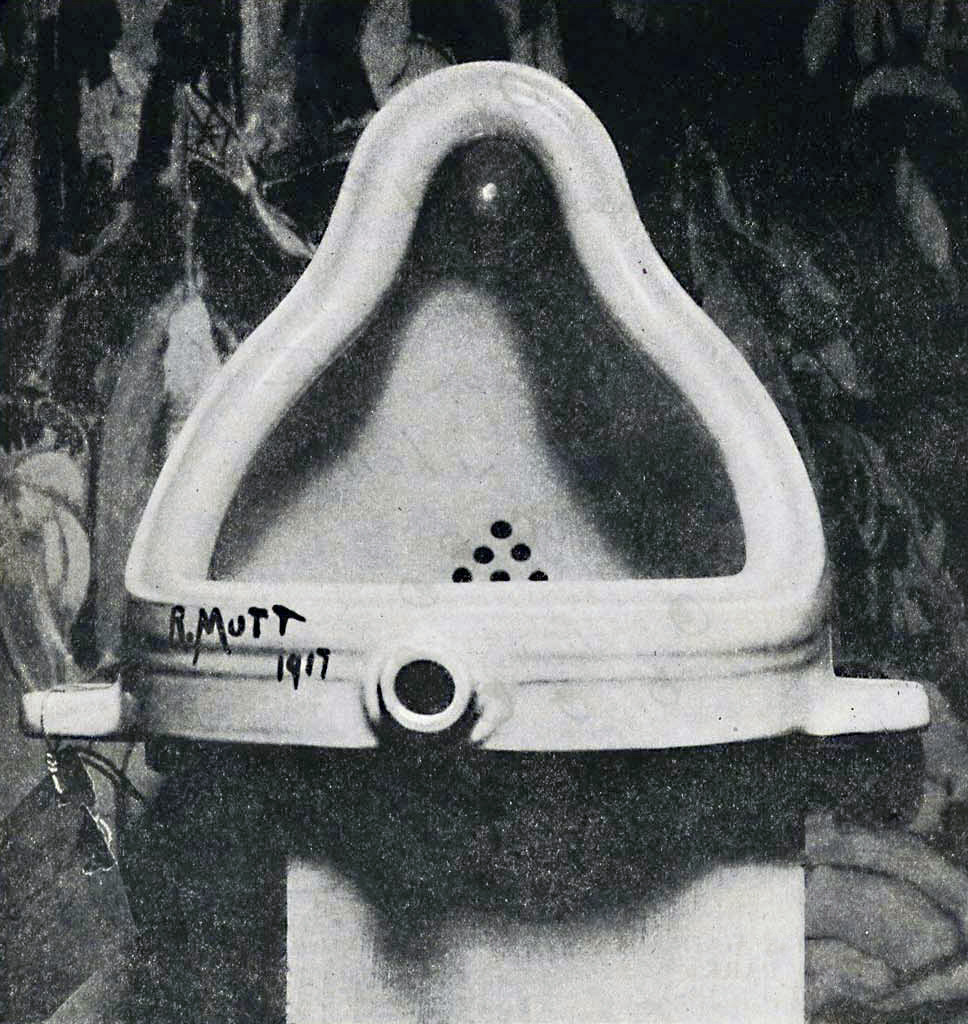
\includegraphics[width=\textwidth]{graphics/Duchamp_Fountaine.jpg}
    \caption{Marcel Duchamp, \textit{Fountain}, 1917, Porcelain urinal}
    \label{fig:Duchamp_Fountaine03}
  \end{minipage}
\end{figure}
%........................................


\end{document}